\chapter{Datenmodellierung} % (fold)
\label{sec:datamodelling}
Um für das empirische Experiment eine Datenbasis zu schaffen, benötigt es ein Datenmodell. Hierbei soll ein möglichst realistisches und flexibles Modell genutzt werden, das zudem Verzweigungen aufweisen sollte, um verschiedene Anfragekomplexität abbilden zu können. Ein geeignetes Beispiel hierfür bietet ein Projektmanagementtool, das in diesem Szenario als Grundlage dient (vgl. Abb. 4.1). Dieses Tool besteht aus drei Klassen, die über drei Beziehungen miteinander verbunden sind. Die Klasse Person modelliert einen Menschen mit den Attributen \texttt{Firstname, Lastname} sowie \texttt{E-Mail} und steht mit der Klasse \texttt{Project} in einer n:n-Beziehung, wodurch mehrere 
\texttt{Project} Objekte einer \texttt{Person} zugeordnet werden können, aber auch mehrere \texttt{Person} Objekte an einem \texttt{Project} arbeiten können. In der Klasse \texttt{Project} werden nur der \texttt{Title} und das \texttt{Date} gespeichert, an dem das \texttt{Project} erstellt wurde. Ein \texttt{Project} steht in einer 1:n-Beziehung zur Klasse \texttt{Issue}, wodurch einem \texttt{Issue} nur ein \texttt{Project} zugeordnet werden, ein \texttt{Project} aber mehrere \texttt{Issue} Objekte beinhalten kann. Hierbei speichert \texttt{Issue} Daten wie den \texttt{Title}, das \texttt{Date} an dem das \texttt{Issue} erstellt wurde, den \texttt{State} und die \texttt{StateReason}. Weiter besitzt \texttt{Issue} eine n:n-Beziehung zu \texttt{Person}, wodurch ein \texttt{Issue} von mehreren \texttt{Person} Objekten bearbeitet werden und eine \texttt{Person} an mehreren \texttt{Issue} Objekten tätig sein kann.
\vspace{1cm}
\label{sec:datenmodell}
\begin{figure}[h!]
	\centering
	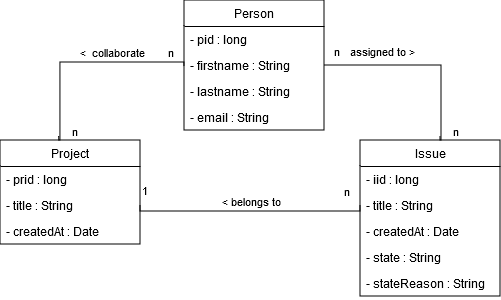
\includegraphics[scale=.8]{Illustrations/class_diagram.png}
	\caption{Klassendiagramm}
\end{figure}


% chapter datamodelling (end)

